\subsection{Formal BON}
\subsubsection{Structure}
Contrary to the structure of the informal specifications described in section \ref{implementation-informal-structure}, the structure imposed on formal specifications is less restrictive. In fact, there are only two restrictions, which will be elaborated upon in the following paragraphs. The reason for this, as already pointed out in section \ref{design-type-system}, is that formal specifications may be used to to give detailed descriptions of a system on the micro-scale, at which point the user probably does not want to recreate the entire system structure.
\paragraph{}
The first restriction is that a class or cluster can be declared as being a part of at most one cluster (zero is allowed). To ensure consistency of the formal specification, checking the cluster structure happens in the same way as for the informal structure: by emitting a type error if the \textit{parent} attribute of a cluster (\textsc{tbon\_tc\_cluster\_type}) or the \textit{cluster} attribute of a class (\textsc{tbon\_tc\_class\_type}) is assigned to more than once.
\paragraph{}
The second restriction is that any cluster structure implied by a static reference must be explicitly defined. This is most easily explained with an example.
\begin{figure}[H]
{\footnotesize
\begin{verbatim}
1| static_diagram STATIC_RELATIONS
2| component
3|       COLLECTIONS.CONTAINERS.LIST inherit SEQUENCE
4| end
\end{verbatim}
}
\caption{Example of static references in use}
\label{fig:structure_static_references}
\end{figure}
In figure \ref{fig:structure_static_references}, an example of static references used in an inheritance relation is shown. For this example to be well-typed, the second restriction says that somewhere in the formal specification, the class \textsc{list} must be defined in a cluster \textsc{containers}, which in turn must be defined as a subcluster of a cluster \textsc{collections}. Interestingly, the static reference on the right, \textsc{sequence}, implies no structure of the system, and could be defined anywhere in the system structure. It would have to be defined somewhere, though.
\subsubsection{Static Relations}
In continuation of the above discussion of static references, static relations constitute a valuable tool for emphasizing or make explicit important relations of the system. As the properties of static references (of which static relations are comprised) have already been attended to, these will not be addressed here. Instead, the specifics of inheritance and client relations, respectively, will be elaborated upon.
\subsubsubsection{Inheritance Relations}
An important thing to note about inheritance relations is that they do not define any previously unknown relations in the system. Their purpose is to emphasize and give more detail to already existing relations. Consequently, any inheritance relation stated in a static diagram must also be expressed in the \textbf{inherit} clause of the class specification of the child class. If it is not stated here, then the parent class must an ancestor to the child class through explicitly stated links. An example of such a relation is seen in figure \ref{fig:structure_static_references}.

Pertaining to inheritance relations is also an optional multiplicity marker, with which the user can underline the number of times the child class inherits from the parent class. As it does not make sense to state an inheritance relation in which the child class inherits less than once from the parent class, this marker is checked to always be greater than zero.
\paragraph{}
Previously mentioned in section \ref{implementation-unresolved-elements} is the aspect that inheritance relations are marked as unresolved, and checked at the end of the second phase of type checking. Thus, provided that the static references of the inheritance relation is well-typed, determining if the relation is well-typed is a matter of checking that the child class exists in the context, and that the parent class is indeed an ancestor to the class through direct inheritance links. This is checked by a call to the feature \textit{conforms\_to} on the child class with the parent class as input. This feature is discussed in the next section concerning the implementation of variance. 
\subsubsubsection{Client Relations}
A client relation between two classes tells a different and possibly more complex story than an inheritance relation. Because \bon{} is a specification language with no knowledge of the actual implementations of the body of a feature, there may very well exist a client relation between to classes in the actual implementation of a system that is not made explicit (e.g. through feature types or feature arguments) in the textual \bon{} specification. Accordingly, the well-typedness of a client relation is not determined on the basis of an explicit client-supplier relation in the specification. In fact, the type checker does not check this aspect at all.
\paragraph{}
Other aspects of a client relation can and should be checked, though. As a consequence of the above, all of these aspects pertain to the client class, as nothing can be said about the supplier, besides that it must be defined.
\begin{figure}[H]
{\footnotesize
\begin{verbatim}
  1| static_diagram CLIENT_RELATIONS
  2| component
  3|    CITIZEN client { drive, cruise, pick_up } CAR "Example 1"
  4|  
  5|    class CAR_OWNER[E] inherit CITIZEN
  6|    CAR_OWNER client { make: E } CAR "Example 2"
  7| 
  8|    GARAGE_NUMBER inherit INTEGER
  9|    CELEBRITY client { cars: MAP[GARAGE_NUMBER, ...] } CAR "Example 3"
 10| end
\end{verbatim}
}
\caption{Examples of client relations}
\label{fig:client_relations}
\end{figure}
%feature names
In particular, the feature names potentially mentioned as client entities in the client relation in question must exist in the interface of the client class. The interface is the set of all the features, including inherited ones, that can be called on a class (see the Features subsection of this section for a more detailed explanation of how the interface is accumulated). Example 1 in figure \ref{fig:client_relations} shows how features can be used in a client relation. All the three features mentioned in this example must be present in the specification of class \textsc{citizen}, which is not shown here, for the client relation to be well-typed.
\paragraph{}
%formal generic names
Accordingly, any formal generic names mentioned as a client entity must exist in the client class as well. This is implemented by a single call to the feature \textit{has\_generic\_name} of \textsc{tbon\_tc\_class\_type}, which iterates through the generics of the class. A formal generic name \textsc{e} is used as a client entity in example 2 in figure \ref{fig:client_relations}. As shown, this formal generic name is present in the class specification of \textsc{car\_owner}.

%named indirection - type parameters must conform
If named indirections are specified as client entities, things become a little more involved. Naturally, every celebrity needs to keep track of his or her cars, even when they are distributed over multiple garages. Example 3 in figure \ref{fig:client_relations} shows how this could be expressed. For this relation to be well-typed, a class \textsc{map} must exist, and it must have two type parameters. Furthermore, \textsc{garage\_number} must conform (covariantly) to the bounding type of the first of these parameters. And because the ellipses refer to the supplier type of the relation \cite[p.~371]{walden1995}, the supplier type must conform to the bounding type of the second parameter. These conformance checks are implemented by calls to the feature \textit{conforms\_to}, the semantics of which are explained next.
\subsubsection{Variance}
\label{implementation-variance}
As described previously in section \ref{design-type-system}, the type checker implements covariant conformance for feature types and feature argument types. Furthermore, as will be seen shortly when generics are discussed, this also holds for instantiation of generic classes with respect to bounding types of generic parameters.
\begin{figure}[H]
{\footnotesize
\begin{verbatim}
 1| conforms_to (other): BOOLEAN
 2|  do
 3|    Result := name of Current is equal to ANY
 4|    if not Result and name of other is not NONE then
 5|       if name of Current is equal to name of other then
 6|         if Current.generic_count = other.generic_count then
 7|              if Current.has_actual_type and other.has_actual_type
 8|                 Result := Current.instance_equality (other)
 9|              elseif Current.has_actual_type xor other.has_actual_type then
10|                 Result := False
11|              else
12|                 Result := Current.generics = other.generics
13|              end
14|         end
15|       else
16|         Result := exists an ancestor a' of Current such that a'.conforms_to(other)
17|       end
18|    end
19|  end
\end{verbatim}
}
\caption{Pseudocode for \textit{conforms\_to}}
\label{fig:conforms_to}
\end{figure}
The conformance check is implemented in the \textit{conforms\_to} feature of \textsc{tbon\_tc\_class\_type}, the pseudocode for which is shown in figure \ref{fig:conforms_to}. Seeing that no other types of variance is implemented anywhere in the type checker, all conformance checks happens through a call to this feature.
Because all classes conform to \textsc{any}, including \textsc{any} itself, the algorithm first checks whether the input is \textsc{any}. If so, nothing remains to be done. Likewise, if the input is \textsc{none}, the algorithm terminates with the result being \textsc{false}.

In all other cases, if the names of the current class and the input are equal, and the number of generics are equal, the algorithms proceeds. If the number of generics are not equal, the two classes can never be equal (even though their names are), because the definition of type parameters is an integral part of the class specification.

Next (on line 7), the algorithms checks whether both the current class and the other class has actual types. The semantics of a call to \textit{has\_actual\_type} on a class are as follows:

{\footnotesize
\begin{center} 
$\exists$ \textit{g} $\in$ \textit{Current.generics} $\mid$ \textit{g:} \textsc{tbon\_tc\_generic} $\bullet$ \textit{g.actual\_type} $\neq$ \textit{Void}
\end{center}}

Thus, if at least one of the generics of the current class has an actual type, the same must hold for the other class. Actual types will be explained in-depth in the Generics subsection of the current section. In this case, instance equality must hold between the two classes. Instance equality is defined as a check that checks whether the actual types of two generic classes are identical. Because, as defined in section \ref{design-type-system}, no conformance relation is considered between two instances of the same generic type with different concrete type arguments, instance equality between two classes only holds if the concrete types are identical.

If only one of the classes have actual types (line 9), they can never conform to each other, as the class with no actual types would represent a class specification, while the other would represent an instance of that class. Accordingly, if neither the current class nor the other class have any actual types, they are both class specifications, and as such, they are considered to be equal if their names are equal and their generics (concerning formal generic names and bounding types of these) are equal (line 12).

In the end (line 16), if the other class is not \textsc{any} or \textsc{none}, and not equal by name to the current class, the algorithms call itself recursively on all the ancestors of the current class, until the entire inheritance hierarchy has been traversed. 
\paragraph{}
As a consequence of the above, one need only to change the logic of \textit{conforms\_to} in order to implement contravariance for feature types, for instance. It should be noted, however, that the current implementation implements covariance for both feature types and feature argument types. Should the variance for these two be inequal in the future, one would need change the feature calls in the type checker accordingly.

Instance equality is implemented in the feature \textit{is\_instance\_equal} in \textsc{tbon\_ tc\_class\_type}. To implement a conformance relation between two instances of the same generic class, one would only need to change the logic of this feature (provided that the implementation of \textit{conforms\_to} remains unchanged). Hence, the logic  for creating a relation between \textsc{list}[\textsc{integer}] and \textsc{list}[\textsc{real}] could be placed here.

\subsubsection{Features}
At the heart of a class specification are its features, the relations of which are discussed in this section. Features are represented in the type checker by the class \textsc{tbon\_tc\_feature}. As mentioned in section \ref{implementation-context-class-structure}, a class in the type context is associated with a set of instances of these. In turn, a feature is associated with its arguments through a list of instances of \textsc{tbon\_tc\_feature\_argument}. 
\subsubsubsection{Feature Status}
Whenever a feature exists in a class specification in which ancestors are specified, it can potentially have a precursor. Luckily, because features repeatedly effect, undefine, and redefine each other all the way down the inheritance hierarchy, only the nearest precursor feature needs to be considered when determining whether a feature specification is well-typed. The status of a feature is implemented by simple boolean flags in \textsc{tbon\_tc\_feature}; and as specified in the grammar in \cite{walden1995}, only one (or none) of these can be set at any given time.
\begin{figure}[H]
    \centerline{\scalebox{0.75}{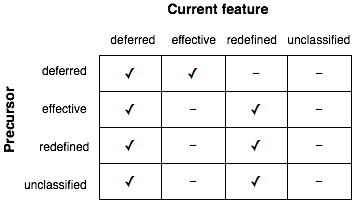
\includegraphics{images/feature_status.png}}}
    \caption[Feature status matrix]{Allowed status relations between a feature and its precursor}
    \label{fig:feature_status}
\end{figure}
Figure \ref{fig:feature_status} shows the allowed relations between the status of the precursor and the status of the current feature (i.e. the feature whose well-typedness is being determined). Notably, what it shows is that it is always possible to undefine an inherited feature by creating a \textit{deferred} version of it in the current class, regardless of the status of the precursor. This becomes relevant in any situation in which one wants to ensure that all concrete descendants of the current class redefines (or, more precisely, effects) the undefined feature.

As for the \textit{effective} status, the restrictions for it may seem overly constraining at first, when considering that the original specification of it states that "[the effective marker] may also be used just to emphasize that the feature will have an implementation," \cite[p.~40]{walden1995}. However, figure \ref{fig:feature_status} only status that \emph{if} a precursor exists for an \textit{effective} feature, then it must be \textit{deferred}. If no precursor exists, one may use it freely.

The \textit{redefined} status is defined as one would expect from the definition in \cite[p.~40]{walden1995}. The only noteworthy aspect is that if a precursor is \textit{deferred}, the current feature must be marked as \textit{effective}, as conceptually, one cannot redefine something that has yet to be defined.

For unclassified features, the definition is straightforward: an unclassified feature defined in the current class can never have a precursor. An unclassified feature inherited from an ancestor can be redefined and undefined as expected, though.
\subsubsubsection{Detecting Duplicate Features}
 This interface is accumulated by traversing the inheritance hierarchy from the bottom up, adding to the interface set any feature with a unique name, or any feature that could lead to duplicate feature names in the interface. The latter are added to give the type checker an opportunity to emit error messages 
\begin{itemize}
\item Has a name that is not already in the interface, or
\item Has the same name as a known feature in the interface, and is on the \emph{same} level in the inheritance hierarchy as the known feature. Or,
\item Has the same name as a known feature in the interface, and is on a \emph{higher} level in the inheritance hierarchy as the known feature, and has a type that does \emph{not} conform to the type of the known feature.
\end{itemize}
The features at level 0 are the local features of the class in question - all other features have a level greater than 0, and are inherited. While the first point should make sense, the two other require some explanation. Because the type checker needs to be able to emit error messages for duplicate features in the inheritance hierarchy, features with identical names on the same level are included. Likewise, if a feature is higher up in the inheritance hierarchy and has a type that does not conform to the type of the already known feature with the same name, it is also included in the interface. This allows the type checker to detect that the inherited feature is not a precursor to an already existing feature, and thus must be a duplicate.
\subsubsubsection{Aggregation}
\cite{ostroff2001}
\subsubsubsection{Prefix and Infix Features}
For regular features, having two features with identical names in the same class (either directly defined in the class or inherited) is not allowed; this is not true for prefix and infix features. For instance, it should be possible to define the operator ''+'' as both a unary and a binary operator on an object, e.g. an integer. The really interesting aspects of prefix and infix features arises when they are used, though, which will be described in the Formal Assertions subsection of the section.

\subsubsection{Generics}
\label{implementation-generics}
In textual \textsc{bon}, formal specifications can involve generics in several different ways:
\begin{itemize}
\item Class specifications, e.g. \textsc{list}[\textsc{e}]
\item References to formal generic names of enclosing class,\newline e.g. \textit{first\_element}: \textsc{e}
\item Generic class specifications instantiated with concrete types,\newline e.g. \textit{string\_list}: \textsc{list}[\textsc{string}]
\item Generic class specifications instantiated with formal generic names of enclosing class, e.g.  \textit{element\_list}: \textsc{list}[\textsc{e}]
\end{itemize}
Note that the first and the last example both refer to \textsc{list}[\textsc{e}], but in very different respects: the former is a specification of a new class \textsc{list} with one (unbounded) type parameter \textsc{e}, while the latter is an instantiation of the same class, in which it is assumed that the enclosing class of the feature \textit{element\_list} has a (possibly bounded) type parameter \textsc{e}. How each of these types of generics are handled by the type checker is explored in this section.
\subsubsubsection{Generics in Class Specifications}
%Generics - explain association between bounding type and actual type.
As mentioned in section \ref{implementation-context-class-structure}, classes in the context are associated with type parameters through a sequence of instances of \textsc{tbon}\_\textsc{tc}\_\textsc{generic}. The class \textsc{tbon}\_\textsc{tc}\_\textsc{generic} has two notable attributes: \textit{bounding\_type} and \textit{actual\_type}. The attribute \textit{bounding\_type} represents the type bound of the formal generic name of the type parameter. Accordingly, the \textit{actual\_type} represents the concrete type associated with the formal generic name.

\begin{figure}[H]
{\footnotesize
\begin{verbatim}
1| static_diagram
2| component
3|       class NUMBER_LIST [E -> REAL]
4| end
\end{verbatim}
}
\caption{Example of a generic class specification with type bounds}
\label{fig:generic_class_specification_bounded}
\end{figure}

In the type context, no generic class specifications have any actual types associated with any of its type parameters; these are only present in instances of these, which will be discussed next. To exemplify, consider the case presented in figure \ref{fig:generic_class_specification_bounded}. Here, the class \textsc{number\_list} would exist in the type context, and have a single type parameter with a formal generic name \textsc{e} and a \textit{bounding\_type} attribute pointing to the type \textsc{real} (which would also exist in the type context in order for the specification to be well-typed). The \textit{actual\_type} attribute of the type parameter would point to \textit{Void}, as this example is not an instantiation of the type in question, but a specification.

As a result of this, and to differentiate between them, there is no equivalence relation between a class specification (without any actual types) and an instance of this class (with actual types), as they in practice are two different types. They are not unrelated, however, as will be explained next.
\subsubsubsection{Instantiation of Generic Types}
Because a generic class specification only specifies a family of concrete classes that have a common base type,  it has to be instantiated with concrete types to be of any practical use.  One could say that a generic class specification merely acts as a template for such concrete instances (in some languages, such as C++, generic classes are explicitly denoted \textit{templates} \cite{stroustrup1997}), and therefore it is not possible to refer directly to a generic class specification in places where a concrete type is expected; in textual \textsc{bon}, these places include feature types, feature argument types, formal assertions, and interestingly, type bounds in generic class specifications. In order to instantiate a generic type, a mechanism that ambiguates between the generic class specification and an instantiation of it is needed, while still ensuring that the instantiated type has all the same attributes (e.g. features) of the generic class specification.
\paragraph{} All types eligible for participation in the instantiation of a generic type are found in the type context after the first phase. Whenever an instantiation of such a type occurs, for instance as a feature type, the type checker [...]:
\begin{enumerate}
\item Creates a deep copy of the generic class
\item Registers the copy in the generic class as an instance of that class
\item Adds the concrete type parameters as actual types to the generics of the copied class
\end{enumerate}
In practice, the first two steps happen as a single call to the \textit{new\_instance} feature of the generic class, the specification of which is found in the type context. As such, the individual instantiations of a generic class are not added directly to the type context. Instead, each generic class keeps track of all the instantiations that have been made of it. The benefit of this approach is that whenever the generic class is updated, i.e. an ancestor or a feature is added in the second phase, the generic class can update all of the instantiations of it accordingly. Consequently, when an instance is registered as an instance (step 2 in the above enumeration), one can think of it as an observer observing the generic class, which then notifies/updates the instantiations whenever a change occurs.
\paragraph{} In step 1 above, it is noted that a \emph{deep} copy is created. This is an important aspect because, as previously explained, type parameters of a class are implemented by associating a type with a sequence of instances of \textsc{tbon}\_\textsc{tc}\_\textsc{generic}. If only a shallow copy was created, the copy would refer to the exact same type parameters as the original, thus making it impossible to add individual concrete actual types to each of these parameters for each instance without affecting the original generic specification.
\subsubsubsection{References to Generic Types}
The instantiation of generic classes explained above happens every time a reference to a concrete type is expected and a generic type is provided in the abstract syntax.
\begin{figure}[H]
{\footnotesize
\begin{verbatim}
1| static_diagram
2| component
3|       class MAP [K -> INTEGER, V]
4|       class MAP_CLIENT
5|          feature
6|             string_map: MAP [INTEGER, STRING]
7|          end
8| end
\end{verbatim}
}
\caption{Example of a reference to a generic type}
\label{fig:ref_generic_type}
\end{figure}
In the example in figure \ref{fig:ref_generic_type}, an instantiation of the generic type \textsc{map} is shown. At the time the type checker resolves the feature \textit{string\_map} (at the end of the first phase), the generic class specification (with no actual types, although the first type parameter has a type bound of type \textsc{integer}) of the type \textsc{map} exists in the type context. To resolve the feature, the resolving code recognizes that \textsc{map} has type parameters, and therefore creates a new instance of \textsc{map} to which the feature can refer (steps 1 and 2 in the previous section). Furthermore, the concrete type \textsc{integer} is added as actual type to the first parameter of the new instance, and \textsc{string} is added as actual type to the second parameter. As such, the feature  \textit{string\_map} now refers to a separate instance of \textsc{map}, which has all the features of the generic class from which it originates plus the added actual types.
%Covariant conformance between bounds
\paragraph{} In order for this new instance to be well-typed, the type of the first concrete parameter type must conform covariantly to the bounding type of the first parameter of the class specification, \textsc{k} (just as defined for feature types and feature argument types in section \ref{design-type-system}). Textual \textsc{bon} has no construct for differentiating between different types of variance for type parameters, which is known from languages such as Java and C\#, and enforcing covariant conformance is thus a design decision on the part of the type checker. This decision mainly based upon the fact that the Eiffel language also enforces covariant conformance of type parameters \cite[Constrained~genericity]{meyer2001}. Future versions could include a switch to fine-tune this aspect of type checking.

As described in section \ref{implementation-variance}, this conformance check also happens through the feature \textit{conforms\_to}. In the presented example, the concrete type trivially conforms to the bounding type, as they are both \textsc{integer}. Some non-trivial situations, however, require a little more consideration.
\subsubsubsection{Solutions to Non-trivial Generics Situations}
The first non-trivial situation considered is presented in figure \ref{fig:non_conforming_type_bounds}.
\begin{figure}[H]
{\footnotesize
\begin{verbatim}
1| static_diagram
2| component
3|    class SEQUENCE [G -> REAL]
4|    class CLIENT_CLASS [H]
5|       feature
6|          seq: SEQUENCE [H]
7|       end
8| end
\end{verbatim}
}
\caption{Situation 1) Example of non-conforming type parameter bounds}
\label{fig:non_conforming_type_bounds}
\end{figure}
In this example, the feature \textit{seq} instantiates the class \textsc{sequence} with the type parameter \textsc{h} of the enclosing class \textsc{client\_class}. The type parameter of \textsc{sequence} is bounded by \textsc{real}, while the parameter \textsc{h} has no bound; so how can it be determined if \textsc{h} is a legal parameter, which makes the instantiation well-typed? Intuitively, one might say that if the type parameter has no bounding type, nothing at all can be said about it -- it could be anything. And by following that intuition, the answer is given: if \textsc{h} has no explicit bounding type, it is implicitly bounded by \textsc{any}, which is the base class of all classes. This mimics the behaviour found in Eiffel, in which unconstrained type parameters are also considered to be bounded by \textsc{any} \cite[p.~77]{meyer2001}.

Now, is the example then well-typed? No, because the concrete type parameter of an instantiation must conform to the bounding type of the type parameter in the class specification, and the only thing known about \textsc{h} is that it has type \textsc{any}, the example is not well-typed, as \textsc{any} does not conform to \textsc{real}.
\paragraph{} The second situation contain similar, but different, subtleties.
\begin{figure}[H]
{\footnotesize
\begin{verbatim}
1| static_diagram
2| component
3|    class SEQUENCE[G]
4|    class A [E -> SEQUENCE[REAL]]
5|    class B [M -> SEQUENCE[INTEGER], N -> A[M]] 
6| end
\end{verbatim}
}
\caption{Situation 2) Specification of a generic class with generic type bounds}
\label{fig:generic_type_bounds}
\end{figure}
Firstly, the differences between the three instantiations of the class \textsc{sequence} should be noted (also note that in this example, the type parameter of \textsc{sequence} has no bounding type). Secondly, the example shows a type parameter \textsc{n} that is bounded by a generic class \textsc{a} instantiated with the first parameter of class \textsc{b},  \textsc{m}. Instantiating a bounding type with another type parameter is permitted, as long the type parameter used in the instantiation is declared at the time of its use (i.e. the type parameter appears to the left of the type parameter that uses it in its specification).

What happens in this case is that \textsc{m} is considered to be a sequence of \textsc{integer}, while the type parameter of \textsc{a} is bounded by a sequence of {real}. At the time of the instantiation of class \textsc{a} for the bound of type parameter \textsc{n}, the bounding type of \textsc{m} has to conform to the bounding type of \textsc{a} in order for the instantiation to be well-typed. But, as already defined in section \ref{design-type-system}, the type checker does not consider a sequence of \textsc{real} to conform to a sequence of \textsc{integer}, even though \textsc{integer} might be a subtype of \textsc{real}. Consequently, to make this situation well-typed, one would have to change the bounding type of either type parameter \textsc{e} or \textsc{m}, such that they become equal.

\subsubsection{Formal Assertions}
\label{implementation-formal-assertions}
% variable context
TEXT
\subsubsubsection{Variable Context and Scope}
For keeping track of the variables introduced in a quantification, a variable context is introduced. This context is implemented as a hash table mapping a variable name to an instance of \textsc{tbon\_tc\_class\_type}.

For the reason that the grammar in \cite{walden1995} specifies that variables can only be introduced in member  or type range expressions in a quantification, discussing variable scope is only relevant for these. The implemented scoping rules for quantifications defines all variables in the same assertion clause to have the same scope. Hence, two boolean expressions in two distinct assertion clauses have distinct scopes.
\begin{figure}[H]
{\footnotesize
\begin{verbatim}
 1| static_diagram
 2| component
 3|  class A
 4|   feature
 5|     list_one: LIST[INTEGER]
 6|     list_two: LIST[INTEGER]
 7|   invariant
 8|     for_all i member_of list_one such_that i: INTEGER it_holds 
 9|       exists i member_of list_two such_that i: INTEGER it_holds i = i; 
10|         -- The above introduces ambiguity;
11|     exists i member_of list_one such_that i: INTEGER it_holds i = 7; 
12|         -- This is fine
13| end
\end{verbatim}
}
\caption{Example of consequence of nested scoping}
\label{fig:variable_scoping}
\end{figure}
The consequence of this definition is that no local scope exists for individual quantification expressions within the same assertion clause. Allowing local scope would mean that the first assertion clause (lines 8-9) in the invariant in figure \ref{fig:variable_scoping} would be well-typed. However, the proposition of the existential quantification of the first assertion clause leaves ambiguity between the origin of the two occurrences of the variable \textit{i}. Do they both represent the inner \textit{i}, in which case the proposition is a tautology? Or does one of them represent the outer \textit{i}? Disambiguation is impossible. Although it could have been decided to implement hiding, in which the second definition of \textit{i} would hide the first definition, this is deemed unnecessary and thus disallowed. There is rarely a reason for insisting on having identical variable names in a nested quantification, especially if the consequence is less expressive power due to the loss of access to hidden variables. Also, as seen on line 11 in the example, it is quite possible to use the same variable again in one of the other assertion clauses of the invariant.
% operator expressions
\subsubsubsection{Operator Expressions}
Operator expressions are expressions involving unary or binary operators. Although the grammar in \cite{walden1995} specifies than an operator can also be an arbitrary parenthesized boolean expression, this specification has been reworked as described in section \ref{design-grammar-deviations} in order for the grammar to type check. 
\paragraph{}
As previously mentioned in the Features subsection, unary/prefix and binary/infix operators are implemented as instances of \textsc{tbon\_tc\_feature} with either the \textit{is\_prefix} or \textit{is\_infix} flag set (but never both). In consequence, for any operator expression in a formal assertion to be well-typed, a prefix or infix feature for the types involved in the expression must be defined in the system. This is true even for default types (described in section \ref{implementation-standard-types}), for which all operators are implicitly defined in the type context. For unary operators, this (quite obviously) means that the operator must be defined as a prefix feature in the class specification of the operand. For binary expressions, it means that the operator must be defined as an infix feature in the class specification of the \emph{left} operand, and the feature must take a single argument of the type of the \emph{right} operand. This is illustrated in the following example:
\begin{figure}[H]
{\footnotesize
\begin{verbatim}
 1| static_diagram
 2| component
 3|    class A
 4|       feature
 5|         infix "+": INTEGER
 6|           -> other: B  
 7|          b: B
 8|       invariant
 9|         (Current + b) > 0; -- OK;
10|         (b + Current) <= 10; -- Type error!;
11|    end
12|    class B
13| end
\end{verbatim}
}
\caption{Definition and use of an operator expression}
\label{fig:operator_expressions}
\end{figure}
The example in figure \ref{fig:operator_expressions} shows that because the infix feature is defined in class \textsc{a}, and takes a \textsc{b} as its argument, the first expression on line 9 is well-typed. The second expression on line 10 is not, however. For this expression to be well-typed, a similar feature taking an \textsc{a} as its argument would have to be specified in class \textsc{b}. While not implementing symmetry for binary operators may seem restrictive at first, consider that the expression could involve any binary operator. If, for instance, a user were to implement the \textit{member\_of} operator for a custom set type, having both ''\textit{var member\_of} \textsc{set\_type}''  and ''\textsc{set\_type} \textit{member\_of var}'' being legitimate expressions would most likely be undesired.
\paragraph{}
Checking that a binary operator expression is well-typed is implemented by finding the corresponding infix feature in the interface of the class of the left operand and checking that the type of the right operand conforms to the type of the feature argument (by a call to \textit{conforms\_to}). For unary expressions, the prefix feature corresponding to the operator must merely be present in the interface of the type of the operand. 
% calls
\subsubsubsection{Calls}
Determining which calls are allowed to be made in an assertion clause depends on where the assertion clause is placed. The first call in a call chain of a call in a feature contract can be to any feature in the interface of the enclosing class (aside from the current feature itself) or to any of the arguments of the current feature. If in a class invariant, only the features in the interface of the current class can be called as the first call in the call chain. These are the rules for calls without a parenthezised qualifier. Is a parenthesized qualifier present, only the features in the interface of the type of the parenthesized qualifier expression can be invoked as the first call.

Beyond the first call in the call chain, the general rule is that a feature that is called as call \textit{n} in the call chain must be in the interface of the type of call \textit{n-1}. This is clarified by the following example:
\begin{figure}[H]
{\footnotesize
\begin{verbatim}
 1| static_diagram
 2| component
 3|  class A
 4|    feature
 5|       infix "+": B
 6|          -> other: B
 7|          require
 8|             other /= Void
 9|          ensure
10|            Result.id = 10
11|          end
12|        b: B
13|    invariant
14|      b /= Void;
15|      (Current + b).id > 5
16|    end
17|  
18|  class B
19|    feature
20|       id: INTEGER
21|    end
22| end
\end{verbatim}
}
\caption{Using calls in assertions}
\label{fig:call_assertions}
\end{figure}
Figure \ref{fig:call_assertions} shows several interesting aspects. First of all, it shows that feature arguments should be accessible from pre- and postconditions of a feature and that attributes of the type of a feature should be accessible through the \textit{Result} keyword. A more subtle point is shown on line 15: because the ''+'' operator called with \textit{Current} as left operand and \textit{b} as right operand returns a type \textsc{b}, the feature \textit{id} of \textsc{b} is available for comparison in the invariant of \textsc{a}. In fact, disregarding equality checks, the only feature that can be called on the parenthesized qualifier on line 15 is \textit{id}, as this is the only feature of \textsc{b}.
\paragraph{}
Type checking calls is done by resolving the type of the call or the parenthesized qualifier through a call to the feature \textit{type\_of\_expression} in the type checker, the details of which are explained later in this section. When the type has been resolved, it is checked that only allowed features are called on the resolved type. Does the call involve features with arguments, the concrete types given as actual arguments must conform to the types specified in the specification of the feature in question (checked through \textit{conforms\_to}).
\paragraph{}
Besides the uses that have already been shown, calls can also participate in set expressions, at which point an extra layer of checking is added to them. This, amongst other issues of type checking set expressions, is discussed next.
% set expressions
\subsubsubsection{Set Expressions}
\label{implementation-set-expressions}
\paragraph{Enumerated sets}
\paragraph{Calls and operator expressions}
TEXT
% getting the type of an expression
% Feature pre- and postconditions vs. invariants
\subsubsubsection{Resolving the Type of an Expression}
% boolean types and quantifications
\subsubsubsection{Quantifications and Boolean Types}
\label{implementation-def-boolean-type}